% Created 2019-06-27 四 09:23
% Intended LaTeX compiler: xelatex
\documentclass[presentation]{beamer}
\usepackage{graphicx}
\usepackage{grffile}
\usepackage{longtable}
\usepackage{wrapfig}
\usepackage{rotating}
\usepackage[normalem]{ulem}
\usepackage{amsmath}
\usepackage{textcomp}
\usepackage{amssymb}
\usepackage{capt-of}
\usepackage{hyperref}
\usepackage{ctex}
\usetheme{default}
\usecolortheme{}
\usefonttheme{}
\useinnertheme{}
\useoutertheme{}
\author{厦门大学公共事务学院}
\date{\today}
\title{一般统计方法的操作}

\hypersetup{
 pdfauthor={厦门大学公共事务学院},
 pdftitle={一般统计方法的操作},
 pdfkeywords={},
 pdfsubject={},
 pdfcreator={Emacs 26.2 (Org mode 9.1.9)}, 
 pdflang={English}}
\begin{document}

\maketitle

\section{概率分布}
\label{sec:orga0c69b4}
\begin{frame}[label={sec:org715bbf1}]{概率基础知识}
概率:在随机试验中,某个结果所代表的事件发生的可能性。在实践中经常用频率来近似表示概率。

如果A, B代表可能的结果, \(P(\bar{A}) = 1 – P(A)\).  
如果A和B是截然不同的结果(不重叠),那么 \(P(A\cup B) = P(A) + P(B)\). 

存在条件概率: \(P(A \cap B) = P(A)P(B|A)\). 
如果A和B独立,则 \(P(B|A) = P(B)\) ,那么有 \(P(A \cap B) = P(A)P(B)\) .

\alert{2008 美国GSS数据}
\begin{center}
\begin{tabular}{lrrrr}
收入 & 很幸福 & 一般 & 不幸福 & 总计\\
\hline
高于平均 & 164 & 233 & 26 & 423\\
平均 & 293 & 473 & 117 & 883\\
低于平均 & 132 & 383 & 172 & 687\\
总计 & 589 & 1089 & 315 & 1993\\
\end{tabular}
\end{center}
A = 高于平均收入,B = 很幸福  

P(A) = 423/1993 = 0.212 (边际概率),P(not A) = 1 – P(A) = 0.788  

P(B) = 589/1993 = 0.296  

P(B|A) = 164/423 = 0.388 (条件概率)  

P(A \(\cap\) B) = P(A)P(B | A) = 0.212(0.388) = 0.082 (等于 164/1993,联合概率)  

A和B独立吗?
\end{frame}

\begin{frame}[fragile,label={sec:orgfab4d0a}]{频数表与列联表}
 \begin{block}{频数表}
\begin{verbatim}
library(vcd)

attach(Arthritis)
table(Improved)
\end{verbatim}

\begin{verbatim}

The following objects are masked from Arthritis (pos = 3):

    Age, ID, Improved, Sex, Treatment

The following objects are masked from Arthritis (pos = 4):

    Age, ID, Improved, Sex, Treatment

The following objects are masked from Arthritis (pos = 5):

    Age, ID, Improved, Sex, Treatment

The following objects are masked from Arthritis (pos = 6):

    Age, ID, Improved, Sex, Treatment

The following objects are masked from Arthritis (pos = 7):

    Age, ID, Improved, Sex, Treatment

The following objects are masked from Arthritis (pos = 8):

    Age, ID, Improved, Sex, Treatment

The following objects are masked from Arthritis (pos = 9):

    Age, ID, Improved, Sex, Treatment

The following objects are masked from Arthritis (pos = 10):

    Age, ID, Improved, Sex, Treatment

The following objects are masked from Arthritis (pos = 11):

    Age, ID, Improved, Sex, Treatment

The following objects are masked from Arthritis (pos = 12):

    Age, ID, Improved, Sex, Treatment

The following objects are masked from Arthritis (pos = 13):

    Age, ID, Improved, Sex, Treatment

Improved
  None   Some Marked 
    42     14     28
\end{verbatim}
\end{block}

\begin{block}{列联表}
\begin{verbatim}
my <- table(Treatment,Improved)
my
\end{verbatim}

\begin{verbatim}

         Improved
Treatment None Some Marked
  Placebo   29    7      7
  Treated   13    7     21
\end{verbatim}
\end{block}

\begin{block}{转化为比例(概率、条件概率)}
\begin{verbatim}
prop.table(my)
# 行条件概率
prop.table(my,1)
# 列条件概率
prop.table(my,2)
\end{verbatim}

\begin{verbatim}
         Improved
Treatment   None   Some Marked
  Placebo 0.3452 0.0833 0.0833
  Treated 0.1548 0.0833 0.2500

         Improved
Treatment  None  Some Marked
  Placebo 0.674 0.163  0.163
  Treated 0.317 0.171  0.512

         Improved
Treatment None Some Marked
  Placebo 0.69 0.50   0.25
  Treated 0.31 0.50   0.75
\end{verbatim}
\end{block}
\end{frame}

\begin{frame}[fragile,label={sec:org96fa602}]{频数表与列联表}
 \begin{block}{添加边际频数}
\begin{verbatim}
addmargins(my)
# 添加行(列)边际频数
addmargins(my,1)
addmargins(my,2)
\end{verbatim}

\begin{verbatim}
         Improved
Treatment None Some Marked Sum
  Placebo   29    7      7  43
  Treated   13    7     21  41
  Sum       42   14     28  84

         Improved
Treatment None Some Marked
  Placebo   29    7      7
  Treated   13    7     21
  Sum       42   14     28

         Improved
Treatment None Some Marked Sum
  Placebo   29    7      7  43
  Treated   13    7     21  41
\end{verbatim}
\end{block}

\begin{block}{添加边际概率}
\begin{verbatim}
addmargins(prop.table(my))
\end{verbatim}

\begin{verbatim}
         Improved
Treatment   None   Some Marked    Sum
  Placebo 0.3452 0.0833 0.0833 0.5119
  Treated 0.1548 0.0833 0.2500 0.4881
  Sum     0.5000 0.1667 0.3333 1.0000
\end{verbatim}
\end{block}

\begin{block}{列联表的另一种方法}
\begin{verbatim}
xtabs(~Treatment+Improved)
\end{verbatim}

\begin{verbatim}
         Improved
Treatment None Some Marked
  Placebo   29    7      7
  Treated   13    7     21
\end{verbatim}
\end{block}
\end{frame}

\begin{frame}[fragile,label={sec:orgd478bce}]{变量的概率分布}
 概率分布指随机变量可能的结果(或结果区间)及其概率

\begin{block}{离散型变量}
P(y) 表示变量 y 的可能结果和概率
\[0\leq P(y) \leq 1, \sum P(y)=1\]
\end{block}

\begin{block}{连续型变量}
连续型变量的概率分布是取值区间的分配概率。
正态分布:
\begin{itemize}
\item 对称,钟形
\item 以均值 \(\mu\) 和标准差 \(\sigma\) 为中心趋势和分散程度特征
\item 对于所有的正态分布,在 \(\mu\) 的任一个特定数值的标准差内的概率是相同的。(68-95-99.7法则)
\end{itemize}
\begin{verbatim}
par(mar=c(4,4,0.1,0.1))
curve(dnorm,-4,4,yaxs='i')
polygon(c(1,seq(1,4,0.1),4),c(0,dnorm(seq(1,4,0.1)),0),col = "red")
\end{verbatim}

\begin{center}
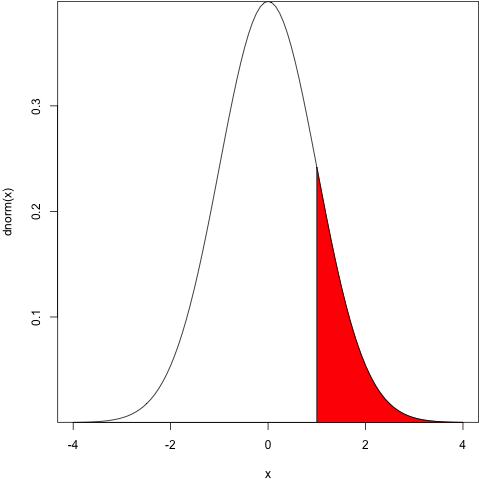
\includegraphics[width=.9\linewidth]{1.png}
\end{center}
\end{block}
\end{frame}

\begin{frame}[label={sec:org1601997}]{正态曲线尾部概率表}
尾部概率:大于 \(\mu + z\sigma\) 的值出现的概率,或距离均值超过z个标准差的值出现的概率  

z的第二个小数点位

\begin{center}
\begin{tabular}{rrrrrrrrrrr}
z & .00 & .01 & .02 & .03 & .04 & .05 & .06 & .07 & .08 & .09\\
\hline
0.0 & .5000 & .4960 & .4920 & .4880 & .4840 & .4801 & .4761 & .4721 & .4681 & .4641\\
\ldots{} &  &  &  &  &  &  &  &  &  & \\
1.4 & .0808 & .0793 & .0778 & .0764 & .0749 & .0735 & .0722 & .0708 & .0694 & .0681\\
1.5 & .0668 & .0655 & .0643 & .0630 & .0618 & .0606 & .0594 & .0582 & .0571 & .0559\\
\end{tabular}
\end{center}

问题: 落在区间 µ - 1.50σ 到  µ + 1.50σ 的概率是多少? 0.072右尾概率对应的z值是多少?  
\alert{\alert{从概率到z值,从z值到概率的变换,要理解清晰,熟练掌握。}}
\end{frame}

\begin{frame}[fragile,label={sec:org47c8145}]{z分数(z-scores)和标准正态分布}
 \begin{itemize}
\item 变量值y的z分数是y离开均值的标准差数: \(z = (观测值-均值)/ 标准差 = (y - \mu )/\sigma\)
\end{itemize}
例子:    y = 65, µ = 50, σ = 10 \(z = (y - \mu)/\sigma = (65 – 50)/10 = 1.5\)  

\begin{itemize}
\item 标准正态分布是均值 µ = 0, 标准差 σ = 1的正态分布

\item z分数和标准正态分布:如果一个变量服从一个正态分布,并且其值通过减去均值和除以标准差被转换为z分数,则z分数服从标准正态分布。
\end{itemize}
\begin{verbatim}
options(digits = 3)
pnorm(65, mean=50, sd=10, lower.tail = FALSE)
pnorm(c(-1.5,1.5))
qnorm(0.072)*(-1)
\end{verbatim}

\begin{verbatim}

[1] 0.0668

[1] 0.0668 0.9332

[1] 1.46
\end{verbatim}
\end{frame}

\begin{frame}[label={sec:orgd79251a}]{抽样分布}
抽样分布:抽样分布展现一个统计量(平均值、标准差等)的可以取的值,以及这些值的概率。

例子:y = 1 如果同意房地产限购政策;y = 0 如果反对

假设样本容量n = 3(注意:抽样次数的区别),考虑样本均值  

\begin{center}
\begin{tabular}{llll}
样本 & 均值 & 样本 & 均值\\
\hline
(1, 1, 1) & 1.0 & (1, 0, 0) & 1/3\\
(1, 1, 0) & 2/3 & (0, 1, 0) & 1/3\\
(1, 0, 1) & 2/3 & (0, 0, 1) & 1/3\\
(0, 1, 1) & 2/3 & (0, 0, 0) & 0\\
\end{tabular}
\end{center}
\end{frame}

\begin{frame}[label={sec:org4f0fb05}]{样本均值的抽样分布}
\begin{itemize}
\item 样本均值 \(\bar y\) 的值随样本的改变而改变,是围绕总体均值 \(\mu\) 波动的变量。
\item \(\bar y\)的抽样分布的标准差被称为 \(\bar y\)的标准误(standard error)。
\item 假定从均值 \(\mu\) 和标准差 \(\sigma\) 的一个总体中抽取容量为n的一个随机样本。 \(\bar y\) 的抽样分布给出 \(\bar y\)的可能值的概率。它的均值为 \(\mu\) ,标准误为:
\end{itemize}
\(\sigma_{\bar y}=\frac{\sigma}{\sqrt n}=\frac{总体标准差}{\sqrt{样本容量}}\)   
\begin{itemize}
\item 实践的意义:在实际研究中,关于相同主题的研究,由于不同的样本,也可能导致研究结果的不同。
\end{itemize}
\end{frame}
\begin{frame}[fragile,label={sec:org96f6152}]{中心极限定理}
 中心极限定理:对于大样本量n的随机抽样,样本均值 \(\bar y\) 的抽样分布是一个近似的正态分布  。

\begin{itemize}
\item 抽样分布的近似正态适用于总体分布的任何形态。
\item 在抽样分布是钟形分布之前n必须有多大,这很大程度上取决于总体分布的偏斜程度。
\item 通过重复选取随机样本,对每个n个观测值的样本计算 \(\bar y\),可以从经验上验证中心极限定理。
\item 中心极限定理意味着:当一个变量是许多个别因素产生的平均结果(没有主导因素)的时候,那么这个变量的分布是接近正态的(例如智商、血压)。
\item 实践中,我们并不知道总体均值 \(\mu\) ,但是我们能够采用抽样分布的离散情况来作为推断未知参数的基础。
\end{itemize}
\begin{verbatim}
par(mar=c(3,4,0.1,0.1),mfrow=c(4,4))
set.seed(1234)
n <- c(2,10,30)
curve(dunif,-0.1,1.1,yaxs='i',ylim=c(0,1.5),xlab = "",ylab = "uniform")
samplemean <- NULL
for(k in n){
  for (i in 1:10000){
    samplemean[i] <- mean(runif(k))
  }  
plot(density(samplemean),main = "",xlab = "",ylab = "")
}
plot(c(0,1,2),dbinom(c(0,1,2),2,0.3),type="h",yaxs='i',xlab = "",ylab = "binomial",xlim=c(-0.5,2.5),ylim = c(0,0.6))
samplemean <- NULL
for(k in n){
  for (i in 1:10000){
    samplemean[i] <- mean(rbinom(k,2,0.3))
  }  
  plot(density(samplemean),main = "",xlab = "",ylab = "")
}
curve(dlnorm,0,10,yaxs='i',xlab = "",ylab = "lognorm")
samplemean <- NULL
for(k in n){
  for (i in 1:10000){
    samplemean[i] <- mean(rlnorm(k))
  }  
  plot(density(samplemean),main = "",xlab = "",ylab = "")
}
curve(dnorm,-4,4,yaxs='i',xlab = "",ylab = "normal")
samplemean <- NULL
for(k in n){
  for (i in 1:10000){
    samplemean[i] <- mean(rnorm(k))
  }  
  plot(density(samplemean),main = "",xlab = "",ylab = "")
}
\end{verbatim}

\begin{center}
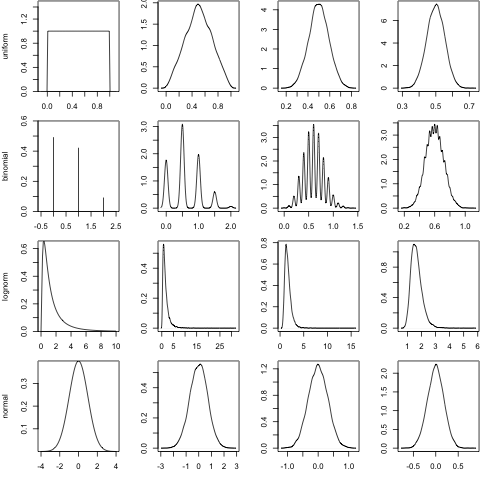
\includegraphics[width=.9\linewidth]{2.png}
\end{center}

由左到右为:总体分布、抽样分布(2)、抽样分布(10)、抽样分布(30)
\end{frame}


\section{统计推断:估计}
\label{sec:org754f3c9}
\begin{frame}[label={sec:org468541a}]{参数估计}
\begin{itemize}
\item 目标:如何利用样本数据估计总体参数的值
\item 点估计:是对参数进行最佳推测的一个数值。
\item 区间估计:是以点估计为中心的一个数值区间,参数值被认为落在其中。
\end{itemize}
\end{frame}

\begin{frame}[label={sec:org6a9b3dd}]{点估计}
\begin{itemize}
\item 利用样本均值估计总体均值 \(\mu\)
\end{itemize}
\[\hat \mu=\bar y=\frac{\sum y_i}{n}\]

\begin{itemize}
\item 利用样本标准差估计总体标准差 \(\sigma\)
\end{itemize}
\[\hat \sigma=s=\sqrt{\frac{\sum (y_i-\bar y)^2}{n-1}}\]
\begin{itemize}
\item 利用样本比例 $\backslash$(\hat \(\pi\)$\backslash$] 估计总体比例 \(\pi\)
\end{itemize}
\end{frame}

\begin{frame}[label={sec:org58143b2}]{好估计量具有的性质}
\begin{itemize}
\item \alert{无偏的:} 估计量的抽样分布以参数为中心
\end{itemize}
e.g. 有偏的估计量:样本全距
\begin{itemize}
\item \alert{有效的:} 与其他估计量相比,具有尽可能小的标准误
\end{itemize}
e.g. 如果总体分布是对称的,并且接近正态,样本均值比样本中位值在估计总体均值和中位值时,更有效
\end{frame}

\begin{frame}[label={sec:org6a9518c}]{置信区间(Confidence Intervals)}
\begin{itemize}
\item 参数的置信区间是一个相信参数落在其中的数值区间。
\item 这种方法产生一个包含参数的区间概率称为置信水平。大多数研究采用的接近1的置信水平,例如0.95或者0.99.

\item 置信区间的形式:
\end{itemize}
$$点估计 \pm 误差边际$$

\begin{itemize}
\item 误差边际是由点估计的抽样分布的离散程度决定的。
\end{itemize}

e.g. 构造拥有“95\%置信度”的一个置信区间,可用点估计加减约两个标准差的误差边际。
\end{frame}

\begin{frame}[label={sec:org1c7c799}]{比例的置信区间}
\begin{itemize}
\item 当 \(y = 1\) 代表感兴趣类别的一个观测值时, \(y = 0\) 就代表另外的观测值,样本比例 \(\hat \pi\) 是一个均值。

\item 总体比例 \(\pi\) 是下面分布的均值
\end{itemize}
$$P(1)=\pi \\ P(0)=1-\pi$$

\begin{itemize}
\item 这个概率分布的标准差是:
\end{itemize}
$$\sigma =\sqrt{\pi (1-\pi )}$$

\begin{itemize}
\item 样本比例 \(\hat \pi\)的标准误是:
\end{itemize}
$$\sigma_{\hat \pi}=\sigma / \sqrt{n}=\sqrt{\pi (1-\pi ) / n}$$
\end{frame}

\begin{frame}[label={sec:org4011502}]{比例的置信区间}
\begin{itemize}
\item 对于大的随机样本,样本比例的抽样分布是接近正态的(中心极限定理)

\item 那么,样本比例 \(\hat \pi\) 应以0.95的概率落在其均值(总体比 \(\pi\))的两个标准差(准确值是1.96)之内。
\end{itemize}
$$\hat \pi \quad 落在 \quad \pi - 1.96\sigma_{\hat \pi} \quad 和 \quad \pi + 1.96\sigma_{\hat \pi} \quad 之间$$

\begin{itemize}
\item 一旦选取了样本,那么有95\%的信心,
\end{itemize}
$$\hat \pi - 1.96\sigma_{\hat \pi} \quad 到 \quad \hat \pi + 1.96\sigma_{\hat \pi} \quad 之间包含 \quad \pi$$
此即总体比例的置信区间。

\begin{itemize}
\item 由于样本比例的标准误含有未知参数,用估计值代替
\end{itemize}

$$se=\sqrt{\hat \pi (1- \hat \pi )} \qquad 替代 \qquad  \sigma_{\hat \pi}=\sqrt{\pi (1-\pi ) / n}$$


\begin{itemize}
\item 对 \$\(\pi\)\$的95\%的置信区间为:
\end{itemize}
$$\hat \pi - 1.96(se) \qquad 到 \qquad \hat \pi + 1.96(se)$$
\end{frame}

\begin{frame}[label={sec:org85c81ca}]{置信区间的性质}
\begin{itemize}
\item 置信区间的宽度随置信水平的增大而增大;随样本量的增大而变小。

\item 置信区间是长期正确的比例.

\item 区间估计方法产生不包括参数的置信区间的概率被称为错误概率 \(\alpha\)

\item \(\alpha = 1- 置信水平\)
\end{itemize}

\begin{center}
\begin{tabular}{lrrr}
\(1-\alpha\) & \(\alpha\) & \(\alpha /2\) & \(Z_{\alpha /2}\)\\
\hline
90\% & .10 & .050 & 1.645\\
95\% & .05 & .025 & 1.96\\
99\% & .01 & .005 & 2.58\\
\end{tabular}
\end{center}
\end{frame}

\begin{frame}[label={sec:orgfc068c7}]{均值的置信区间}
\begin{itemize}
\item 对于大的随机样本,样本均值有渐进正态的抽样分布,其均值为 \$\(\mu\)\$,标准误 \(\sigma_{\bar y}=\sigma / \sqrt n\)

\item 相似的,有 \(P(\mu-1.96\sigma_{\bar y} \leq \bar{y} \leq \mu+1.96\sigma_{\bar y})=0.95\)

\item 有95\%的置信度,样本均值落在(未知)总体均值的1.96个标准误的范围内。

\item 标准误是未知的,因此要用样本数据的点估计来代替标准误
\end{itemize}

$$\bar y \pm 1.96(se), \quad 即 \quad \bar y \pm 1.96\frac{s}{\sqrt n} \qquad se=\frac{s}{\sqrt n}$$

\begin{itemize}
\item 对于较大的样本容量是没有问题的,但是对于较小的样本量,用估计量s替代   \$\(\sigma\)\$会造成误差,置信区间会偏小。因此要采用t分数代替z分数。
\end{itemize}
\end{frame}

\begin{frame}[label={sec:orga1e82be}]{t 分布  (Student’s t from W.S. Gosset)}
\begin{itemize}
\item t分布是钟形分布并关于均值0对称。

\item 标准差略大于1(比标准正态分布的尾部要厚一些)
\end{itemize}
具体形状由自由度(df)决定。对于总体均值的推断,自由度为 df = n – 1 

\begin{itemize}
\item 随着自由度df的增加,t分布越接近于标准正态分布,df大于30时,几乎与标准正态分布相同。

\item t分数(代替z分数)乘以估计的标准误,给出了均值的置信区间的误差边际。
\end{itemize}
\begin{center}

\includegraphics[width=.9\linewidth]{./image1.png}
\end{center}
\end{frame}
\begin{frame}[fragile,label={sec:orgdbd302d}]{部分 t 分数}
 \alert{置信水平}  

\begin{center}
\begin{tabular}{rrrrr}
 & 90\% & 95\% & 98\% & 99\%\\
\hline
df & t.050 & t.025 & t.010 & t.005\\
1 & 6.314 & 12.706 & 31.821 & 63.657\\
10 & 1.812 & 2.228 & 2.764 & 3.169\\
16 & 1.746 & 2.120 & 2.583 & 2.921\\
30 & 1.697 & 2.042 & 2.457 & 2.750\\
100 & 1.660 & 1.984 & 2.364 & 2.626\\
无穷大 & 1.645 & 1.960 & 2.326 & 2.576\\
\end{tabular}
\end{center}

\begin{itemize}
\item df = 无穷大时,和标准正态分布相同。
\end{itemize}
\begin{verbatim}
options(digits=4)
qt(0.025, df=10, lower.tail=FALSE)
\end{verbatim}

\begin{verbatim}

[1] 2.228
\end{verbatim}
\end{frame}

\begin{frame}[label={sec:org9165856}]{总体均值的置信区间}
\begin{itemize}
\item 对于来自正态总体分布的随机样本,均值 \$\(\mu\)\$的95\%置信区间为:
\end{itemize}

$$\bar y \pm t_.025 \times se, \quad 其中 \quad se=s/\sqrt n$$

计算t分数的自由度df = n - 1

\begin{itemize}
\item 正态分布的假定是确保对于任何的n抽样分布都是钟形。

\item \alert{总体均值 \(\mu\) 置信区间的性质}  
\begin{itemize}
\item 对均值的置信区间的假定是:使用随机化选择样本;总体分布是正态的。在这两个假定下,样本均值的抽样分布是正态的。用估计的标准误替代未知的真实标准误后,样本均值服从t分布。

\item 在违背正态总体假定时,对均值使用t分布的置信区间是稳健的(robust)。但是,如果样本数据非常偏态或包含极端异常值,方法的稳健性会降低,因此要进行探索性分析。

\item 置信水平越高,那么置信区间就越大;样本容量 n 越大,置信区间越窄。
\end{itemize}
\end{itemize}
\end{frame}

\begin{frame}[fragile,label={sec:org9461419}]{用R计算置信区间}
 \begin{itemize}
\item 比例的置信区间:1000人的样本中700人选择“YES”,总体比例的95\%的置信区间
\end{itemize}
\begin{verbatim}
y <- 700
n <- 1000
estimate <- y/n
se <- sqrt (estimate*(1-estimate)/n)
int.95 <- estimate + qnorm(c(.025,.975))*se
int.95
\end{verbatim}

\begin{verbatim}

[1] 0.6716 0.7284
\end{verbatim}

\begin{itemize}
\item 均值的置信区间:5个人的年龄组成的样本,总体平均年龄的95\%的置信区间
\end{itemize}
\begin{verbatim}
y <- c(35,34,38,35,37)
n <- length(y)
estimate <- mean(y)
se <- sd(y)/sqrt(n)
int.95 <- estimate + qt(c(.025,.975),n-1)*se
int.95
\end{verbatim}

\begin{verbatim}

[1] 33.76 37.84
\end{verbatim}
\end{frame}

\begin{frame}[fragile,label={sec:org2c8f766}]{置信区间的含义}
 \begin{itemize}
\item 置信区间是长期正确的比例:95\% 的置信度为有95\%的区间会覆盖总体均值 \(\mu\)
\end{itemize}
\begin{verbatim}
# Set the random seed
set.seed(123456)

# initialize vectors to later store results:
CIlower <- numeric(10000); CIupper <- numeric(10000)
pvalue1 <- numeric(10000); pvalue2 <- numeric(10000)

# repeat 10000 times:
for(j in 1:10000) {
  # Draw a sample
  sample <- rnorm(100,10,2)
  # test the (correct) null hypothesis mu=10:
  testres1 <- t.test(sample,mu=10)
  # store CI & p value:
  CIlower[j] <- testres1$conf.int[1]
  CIupper[j] <- testres1$conf.int[2]
  pvalue1[j] <- testres1$p.value
}

# Test results as logical value
reject1<-pvalue1<=0.05

# color vector:
color <- rep(gray(.5),100)
color[reject1[1:100]] <- "black"

# Prepare empty plot with correct axis limits & labels:
plot(0, xlim=c(9,11), ylim=c(1,100), 
		       ylab="Sample No.", xlab="", main="Correct H0")
# Vertical line at 10:
abline(v=10, lty=2)
# Add the 100 first CIs (y is equal to j for both points):
for(j in 1:100) {
  lines(c(CIlower[j],CIupper[j]),c(j,j),col=color[j],lwd=2)
}
\end{verbatim}

\begin{center}
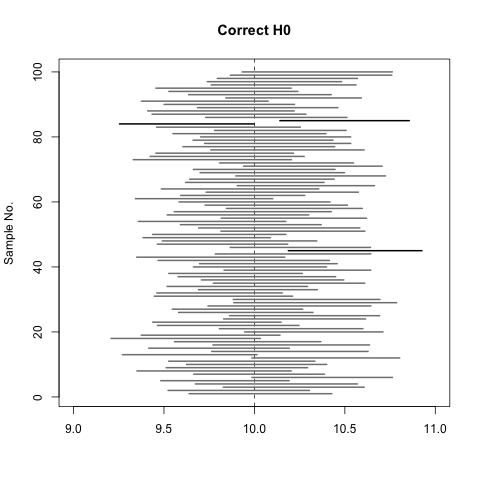
\includegraphics[width=.9\linewidth]{3.png}
\end{center}
\end{frame}

\begin{frame}[label={sec:orgb371788}]{样本量的选择}
\begin{itemize}
\item 在估计总体比例时,选取多大的样本量,才能使得置信度为0.95,误差不超过0.03?

\begin{itemize}
\item 可以让 0.03 = 误差边际,然后求 n 的值

\item \(0.03=1.96\sigma_{\hat \pi}=1.96\sqrt{\pi (1-\pi) / n}\)

\item \(n=\pi (1-\pi)(1.96/0.03)^2=4268\pi (1-\pi)\)

\item \$\(\pi\)=0.5\$时,n值最大,所以 \(n=4268\cdot 0.5\cdot 0.5=1067\)
\end{itemize}
\item 如果从前的研究显示总体均值大概是0.20,95\%置信区间的误差边际为0.03的最低样本量为:
\end{itemize}

$$n=\pi (1-\pi)(1.96/0.03)^2=4268\pi (1-\pi) \\ =4268\cdot 0.2 \cdot 0.8=83$$

\begin{itemize}
\item 总体比例接近0或1的时候,要比总体比例接近0.5更“容易”估计

\item 除非完全不了解总体比例的值,最好是用估计值,而不是0.50计算
\end{itemize}
\end{frame}

\begin{frame}[label={sec:orgd0bccea}]{样本量的选择}
\begin{itemize}
\item 确定估计的参数的类别(总体比例或者总体均值)

\item 选择误差边际 (M) 和置信水平 (决定z分数)

\item 比例(如果不知道,可设 \(\pi=0.50\)):
\end{itemize}

$$n=\pi (1-\pi)(\frac{z}{M})^2$$

\begin{itemize}
\item 均值(需推测总体标准差的值 \(\sigma\)):
\end{itemize}

$$n=\sigma^2(\frac{z}{M})^2$$

\begin{itemize}
\item 置信区间与样本量:

\begin{itemize}
\item 样本量与置信水平(更高的置信度要求更大的样本量)和总体变异度(变异程度越高要求更大的样本量)相关。

\item 实践中,事先确定样本容量比较难。一是因为许多参数都要估计;二是因为资源有限,需要权衡。

\item 任何参数都可以确定其置信区间。
\end{itemize}
\end{itemize}
\end{frame}

\begin{frame}[label={sec:orgb5fe7ab}]{实际使用置信区间时需要考虑的因素}
\begin{itemize}
\item 确定感兴趣的变量类型:
\begin{itemize}
\item 定量变量 – 推断均值
\item 类别变量 – 推断比例
\end{itemize}

\item 检验前提条件是否满足?
\begin{itemize}
\item 随机化 (抽样分布及其标准误)

\item 其他条件?

均值:数据探索性分析检查数据的分布确保均值是一个合适的参数。

比例:类别中的观察个体至少有15个,不在类别中的观察个体也至少15个。
\end{itemize}
\end{itemize}
\end{frame}


\section{统计推断:显著性检验}
\label{sec:org2dfb244}
\begin{frame}[label={sec:orga20f435}]{显著性检验}
\begin{itemize}
\item 目的:利用统计方法检验假设

\begin{itemize}
\item “治疗厌食症,采用认知行为家庭疗法与安慰剂产生的平均体重变化相同”  (没有效果)

\item “社会经济地位越高则心理健康程度越高”  (存在效应)

\item “为别人花钱比为自己花钱更幸福”
\end{itemize}

\item 假设:在统计推断中,对研究所关心的变量,我们会对总体的参数进行某种预测,这种对总体参数的预测便是一个假设。

\item 显著性检验利用样本对参数的点估计与假设预测的参数值之间比较,来评价一个假设。

\item 一般而言我们回答这样一个问题:“如果假设成立,得到现有样本数据的 \alert{不可能性} 有多高?”
\end{itemize}
\end{frame}

\begin{frame}[label={sec:org52ca1c2}]{显著性检验的5个部分}
\begin{enumerate}
\item 前提假定(Assumptions):数据类型(定量数据、分类数据)、抽样方式(随机化)、总体分布(正态分布等)、样本量(是否足够大)

\item 假设(Hypotheses):   
\begin{itemize}
\item 原假设( \(H_0\)):对参数取一个特定值的陈述。(一般是指“没有效果”)
\item 备择假设( \(H_a\)):陈述参数值落在某个备择的值域。(一般指“有效果”)
\end{itemize}

\item 检验统计量:用来和原假设的预测进行比较。一般通过标准误的个数来测量样本点估计与原假设的参数值之间的距离。

\item P值 (P): 用概率来表现的关于原假设成立与否的证据。在原假设成立的条件下,检验统计量等于观测值及更极端值的概率(备择假设预测的方向)。P值越小,那么反对原假设的证据越强。

\item 结论:   
\begin{itemize}
\item 无需判断的话,只报告p值和进行解释。
\item 如需判断的话,选择一个临界点(显著性水平,例如0.05或者0.01)。如果P值小于等于这个临界点的值,那么就拒绝原假设。
\end{itemize}
\end{enumerate}
\end{frame}

\begin{frame}[label={sec:orgd8f86a5}]{均值的显著性检验}
\begin{itemize}
\item 前提假定:随机化,定量变量,正态总体分布(稳健性)

\item 原假设: \$H\(_{\text{0}}\): \(\mu\)=\(\mu_{\text{0}}\)\$,其中 \$\(\mu_{\text{0}}\)\$是总体均值的一个特定的值。
(通常与某个标准相比没有效果或没有变化)

\item 备择假设: \(H_{\alpha}: \mu \neq \mu_0\) 
双侧备择包括大于和小于原假设值

\item 检验统计量: 样本均值离原假设值的距离,用标准误的个数来衡量。
\end{itemize}
$$t=\frac{\bar y-\mu_0}{se}, \quad se=s/\sqrt n$$
当原假设 \$H\(_{\text{0}}\)\$为真,t统计量的抽样分布是自由度为 df = n – 1 的t分布。

\begin{itemize}
\item P值:原假设为真的假定下,t统计量等于观察值或更极端的取值的概率。
对于双侧备择假设 \$H\(_{\alpha}\)\$,那么对应是双尾概率

\item 结论:报告和解释P值,如有需要,还要对原假设 \$H\(_{\text{0}}\)\$进行判断。
\end{itemize}
\end{frame}

\begin{frame}[label={sec:orge1b49f2}]{例子:厌食症的治疗}
\begin{itemize}
\item y为治疗后与治疗前的体重差值:11.4, 11.0, 5.5, 9.4, 13.6, -2.9, -0.1, 7.4, 21.5, -5.3, -3.8, 13.4, 13.1, 9.0, 3.9, 5.7, 10.7
\end{itemize}

\alert{如何证明治疗有效果?}  
\begin{itemize}
\item 设 \$\(\mu\)\$为体重变化的总体均值
\item 检验原假设  \(H_0: \mu=0\)(无效果),相应备择假设 \(H_{\alpha}: \mu \neq 0\).
\item 由数据可以得到
\end{itemize}

\begin{center}
\begin{tabular}{lrrrr}
变量 & 样本量 & 均值 & 标准差 & 均值标准误\\
\hline
体重差 & 17 & 7.265 & 7.157 & 1.736\\
\end{tabular}
\end{center}

$$se=s/\sqrt n=7.157/\sqrt {17}=1.736$$

\begin{itemize}
\item 检验统计量(df=16): \(t=\frac{\bar y - \mu_0}{se}=\frac{7.265-0}{1.736}=4.18\)

\item P值: \(pvalue=2 \times P(t>4.18)=0.0007\)(软件计算)说明如果原假设 \$H\(_{\text{0}}\)\$为真,那么得到一个距离原假设0值至少4.18个标准误远的样本均值的概率为 0.0007。

\item 结论:非常强的证据显示总体均值不为0. (具体看起来 \(\mu >0\))
\end{itemize}
\end{frame}

\begin{frame}[fragile,label={sec:org68de002}]{单样本均值的显著性检验}
 \begin{verbatim}
y <- c(11.4, 11.0, 5.5, 9.4, 13.6, -2.9, -0.1, 7.4, 21.5, -5.3, -3.8, 13.4, 13.1, 9.0, 3.9, 5.7, 10.7)
n <-length(y)
se <- sd(y)/sqrt(n)
t <- (mean(y)-0)/(se)
pvalue <- 2*(1-pt(t,df=16))

t.test(y)
\end{verbatim}

\begin{verbatim}

	One Sample t-test

data:  y
t = 4.1849, df = 16, p-value = 0.0007003
alternative hypothesis: true mean is not equal to 0
95 percent confidence interval:
  3.58470 10.94471
sample estimates:
mean of x 
 7.264706 

\end{verbatim}
\end{frame}

\begin{frame}[label={sec:orge29e3a1}]{双侧检验与置信区间之间的对应关系}
\begin{itemize}
\item 当双侧检验的 P值 \$\(\le\) 0.05\$时,总体均值 \$\(\mu\)\$的95\%的置信区间不包括原假设 \$H\(_{\text{0}}\)\$预测的均值 (例如为0)

\item 上面的例子:P = 0.0007, 95\% 的置信区间为  (3.6, 10.9)

\item 当双侧检验的 P值 > 0.05 时,95\% 的置信区间必然包括原假设 \$H\(_{\text{0}}\)\$预测的均值。

\item 置信区间提供了更多关于总体均值的信息
\end{itemize}

例子: 假设样本均值为7.265、标准差为 7.16都保持不变,但是样本容量 n = 4    (不是前面的 n = 17),那么双侧检验的p值为0.14,95\%的置信区间为(-4.1, 18.7),即p值大于显著性水平,相应置信区间包含了0.
\end{frame}
\begin{frame}[label={sec:orgff2a6b9}]{均值的单侧检验}
例子:
如果研究预测到治疗方法有正面效果,可以采用备择假设 \$H\(_{\alpha}\)>0\$,如果t在右尾部越远,则表明数据越支持这个备择假设,那么此时的P值 = 右尾概率。
\begin{itemize}
\item 假定对于样本 n = 4 (df = 3),有 t = 2.0,那么 \(Pvalue = P(t > 2.0) = 0.07\)
\item 如果备择假设是: \(H_{\alpha}: \mu <0\),  P值 = 左尾概率; \(Pvalue = P(t < 2.0) = 0.93\)
\item 实践中,双侧检验更普遍。
\end{itemize}
\end{frame}

\begin{frame}[label={sec:org45e8c43}]{统计决策}
\$\(\alpha\)\$水平是一个选定的数值,被称为显著性水平。 

如果P值 \$\(\le\) \(\alpha\)\$,那么拒绝原假设 \(H_0\)
如果P值 \$> \(\alpha\)\$,那么不拒绝原假设 \(H_0\) 

注意:表述是“不拒绝 \(H_0\)” 而不是“接受 \(H_0\)”,因为原假设 \(H_0\)  的值仅仅是众多可能取值中的一个。

例子 (n = 4, 双侧): 假定 \(\alpha=0.05\). 由于 P值 =  0.14,那么我们不能拒绝原假设 \(H_0\).  但是 0 仅仅是95\%置信区间 (-4.1, 18.7)的取值中的一个,所以我们只能是不拒绝,不能表述为接受。
\end{frame}

\begin{frame}[label={sec:org964eb13}]{样本量大小对检验的影响}
\begin{itemize}
\item 当样本量 n 比较大时(例如,n > 30),根据中心极限定理,正态总体分布假定变得不重要。

\item 对于小样本量而言,如果正态总体假定不成立,双侧 t 检验是稳健的,然而单侧检验不稳健。

\item 对于给定的观察样本均值和标准差,样本量越大,检验统计量越大(因为分母中的标准误se越小),p值越小

\item 当样本量越大的时候,越可能拒绝一个错误的原假设 \(H_0\)

\item 当样本量较大时,“统计显著性”不等于是“具有实际意义的显著性”
\end{itemize}
\end{frame}

\begin{frame}[label={sec:orgde0cfb3}]{比例的显著性检验}
\begin{itemize}
\item 前提假定:类别变量、随机化、大样本(但是小样本做双侧检验也OK)

\item 假设:
\begin{itemize}
\item 原假设: \(H_0: \pi=\pi_0\)
\item 备择假设: \(H_{\alpha}: \pi \neq \pi_0\)(双侧); \$H\(_{\alpha}\): \(\pi\) > \(\pi_{\text{0}}\)\$或者 \(H_{\alpha}: \pi < \pi_0\)(单侧)
\item 在得到数据前就要设定好假设
\end{itemize}

\item 检验统计量
\end{itemize}

$$z=\frac{\hat \pi-\pi_0}{\sigma_{\hat \pi}}=\frac{\hat \pi-\pi_0}{\sqrt{\pi_0(1-\pi_0)/n}}$$
\begin{itemize}
\item p值:
\begin{itemize}
\item \(H_{\alpha}: \pi \neq \pi_0\) P=标准正态分布双尾概率
\item \(H_{\alpha}: \pi > \pi_0\) P=标准正态分布的右尾概率
\item \(H_{\alpha}: \pi < \pi_0\) P=标准正态分布的左尾概率
\end{itemize}

\item 结论:如果P值小于等于显著性水平,则拒绝原假设 \(H_0\)
\end{itemize}
\end{frame}

\begin{frame}[label={sec:orgaf163ca}]{例子:狗能闻出膀胱癌吗?(British Medical Journal, 2004)}
每次测试,1个膀胱癌尿样放在6个控制尿样中,如何检验狗能否比随机猜测得到更好的结果?

让 \(\pi=\) 某次测试猜对的概率。 \(H_0: \ \pi-1/7\) (= 0.143, 没有影响),  \(H_{\alpha}>1/7\)

54次测试,狗能够做出正确的选择22次。样本比例 = 22/54 = 0.407

标准差 \(se_0=\sqrt{\pi_0(1-\pi_0)/n}=\sqrt{(1/7)(6/7)/54}=0.0476\)

检验统计量: \(z=(\hat \pi-\pi_0)/se_0=(0.407-(1/7))/0.0476=5.6\)

p值=标准正态分布的右尾概率=0.00000001

因此,有非常强的证据显示狗的选择比随机猜测要更好。

那么对于标准的显著性水平 \$\(\alpha\)\$为0.05,我们拒绝原假设 \$H\(_{\text{0}}\)\$得到结论 \(\pi>1/7\).
\end{frame}

\begin{frame}[label={sec:org4180e2a}]{检验中的决策}
\begin{itemize}
\item \$\(\alpha\)\$水平(显著性水平):是一个事先指定的“门槛”,如果P值落在它(一般采用0.05或者0.01)之下,那么拒绝原假设 \(H_0\)

\item 拒绝域:检验拒绝 \$H\(_{\text{0}}\)\$的那些检验统计量值的集合。对于显著性水平 \$\(\alpha\)=0.05\$的双侧检验,如果 \$|z|\(\ge\) 1.96\$,那么拒绝 \(H_0\)

\item 错误类型
\begin{itemize}
\item 第一类型错误:当原假设 \$H\(_{\text{0}}\)\$为真时,拒绝原假设

\item 第二类型错误:当原假设 \$H\(_{\text{0}}\)\$为假时,不拒绝原假设

\item \$\(\alpha\)\$是第一类错误的概率,选择的 \$\(\alpha\)\$越小,则第二类错误发生的概率 \$\(\beta\)\$会增加

\item 检验的功效 = \$1-\(\beta\)\$= P(原假设为假的条件下拒绝它)
\end{itemize}
\end{itemize}
\end{frame}

\begin{frame}[label={sec:orgdb34051}]{正态总体单样本参数假设检验}
\begin{itemize}
\item 总体均值的检验(大样本: \(n \ge 30\))  
\$\(\sigma^{\text{2已知}}\)\$:
\end{itemize}
$$ z=\frac{\bar x-\mu_0}{\sigma/\sqrt{n}}\sim N(0,1)$$
 \$\(\sigma^{\text{2未知}}\)\$:
$$ z=\frac{\bar x-\mu_0}{s/\sqrt{n}}\sim N(0,1)$$
\begin{itemize}
\item 总体均值的检验(正态总体小样本)  
\$\(\sigma^{\text{2已知}}\)\$:
\end{itemize}
$$ z=\frac{\bar x-\mu_0}{\sigma/\sqrt{n}}\sim N(0,1)$$
 \$\(\sigma^{\text{2未知}}\)\$:
$$ t=\frac{\bar x-\mu_0}{s/\sqrt{n}}\sim t(n-1)$$
\end{frame}

\begin{frame}[fragile,label={sec:org76d20db}]{例子}
 某汽车生产商声称其生产的汽车每加仑汽油可行驶的里程不低于25英里,标准差为2.4英里。消协组织了一个由10位汽车主组成的小组,他们的汽车每加仑汽油的可行驶英里数如下表。假定汽车每加仑可行驶里程服从正态分布。现在问,汽车生产商的诺言可信吗?

\begin{center}
\begin{tabular}{lrrrrrrrrrr}
序号 & 1 & 2 & 3 & 4 & 5 & 6 & 7 & 8 & 9 & 10\\
\hline
里程 & 22 & 24 & 21 & 24 & 23 & 24 & 23 & 22 & 21 & 25\\
\end{tabular}
\end{center}
\begin{verbatim}
options(digits = 2)
u.test<-function(x,mu,thegma)
{  se=thegma/sqrt(length(x))
   u=(mean(x)-mu)/se
   p=pnorm(u)
   c(u=u, p=p)
}
b=c(22,24,21,24,23,24,23,22,21,25)
u.test(b, 25,2.4)

\end{verbatim}

\begin{verbatim}
      u       p 
-2.7670  0.0028 
\end{verbatim}
\end{frame}

\begin{frame}[fragile,label={sec:orge67d7f1}]{例子}
 一位投资者考虑是否选择新的资产管理公司,为使收益最大化,如果新的资产公司平均收益率大于原来资产管理公司的平均收益率,公司将选择新的资产管理公司。原来的资产公司的客户平均收益率为50.0\%,对新资产管理公司的客户进行抽样检验,12个客户的收益率如下:50.2\%,49.6\%,51.0\%,50.8\%,50.6\%,49.8\%,51.2\%,49.7\%,51.5\%,50.3\%,51.0\%和50.6\%,假设资产管理公司客户收益率的分布比较近似于正态分布,问新资产管理公司的平均收益率是否大于原来的资产管理公司? 
\begin{verbatim}
x=c(.502,.496,.510,.508,.506,.498,.512,.497,.515,.503,.510,.506)
t.test(x,mu=.500,alternative ="greater") 
\end{verbatim}

\begin{verbatim}

	One Sample t-test

data:  x
t = 2.9564, df = 11, p-value = 0.006529
alternative hypothesis: true mean is greater than 0.5
95 percent confidence interval:
 0.5020609       Inf
sample estimates:
mean of x 
  0.50525 

\end{verbatim}
\end{frame}

\begin{frame}[label={sec:orga529568}]{正态总体单样本参数假设检验}
\begin{itemize}
\item 总体比例的检验  
假定条件:
 总体服从二项分布;
 可用正态分布来近似(大样本)。  

检验的Z统计量:
\end{itemize}
$$ z=\frac{\hat \pi-\pi_0}{\sqrt{\pi_0(1-\pi_0)/n}}\sim N(0,1),\pi_0为假设的总体比例. $$

\begin{itemize}
\item 总体方差的检验  
检验一个总体的方差或标准差,假设总体近似服从正态分布,使用 \$\(\chi^{\text{2}}\)\$分布。  
检验统计量:
\end{itemize}
$$ \chi^2=\frac{(n-1)s^2}{\sigma_0^2}\sim \chi^2(n-1)$$
\end{frame}

\begin{frame}[fragile,label={sec:org945de88}]{总体比例检验示例}
 为调查某大学男女比率是否是1:1,在校门处观察,发现100学生中有45个女性。那么,这是否支持该大学总体男性占比为50\%的假设?
\begin{verbatim}
prop.test(45,100,p=0.5)
\end{verbatim}

\begin{verbatim}

	1-sample proportions test with continuity correction

data:  45 out of 100, null probability 0.5
X-squared = 0.81, df = 1, p-value = 0.3681
alternative hypothesis: true p is not equal to 0.5
95 percent confidence interval:
 0.3514281 0.5524574
sample estimates:
   p 
0.45 

\end{verbatim}
\end{frame}

\begin{frame}[fragile,label={sec:org44a58cd}]{总体方差检验示例}
 某地区环保部门规定,废水经设备处理后水中某种有毒物质的平均浓度,均值和标准差单位是微克。通过抽查20个废水样品,如何判断水样的标准差是否为20微克?
\begin{verbatim}
var.test1<-function(x, sigma2){
  n<-length(x)
  svar=var(x)
  df=n-1
  chi2<-df*svar/sigma2;
  P<-pchisq(chi2,df)
  data.frame(var=svar, df=df, chisq2=chi2, P_value=P)
}
x=c(512.952899108198, 503.85274864927, 495.06951127009, 477.193305294993, 509.400520346022, 493.249014260413, 492.456674317536, 530.078195416527, 498.757258963417, 522.657000900506, 510.041124496973, 490.505063978937, 536.24855605503, 530.039965979141, 495.559165160148, 466.840695851664, 510.702680801237, 524.485012890925, 490.37616974915, 485.579333872921)
var.test1(x,400)
\end{verbatim}

\begin{verbatim}
       var df   chisq2   P_value
1 346.8209 19 16.47399 0.3745438
\end{verbatim}
\end{frame}

\begin{frame}[label={sec:org51bf5c5}]{正态总体双样本参数假设检验}
\begin{block}{双样本方差的检验(方差齐性检验)}
假定条件:
 两个总体都服从正态分布。
 两个独立的随机样本。

检验统计量:
$$ F=\frac{s_1^2}{s_2^2}\sim F(n_1-1,n_2-1)\ 或 \ F=\frac{s_2^2}{s_1^2}\sim F(n_2-1,n_1-1)$$
\end{block}
\end{frame}

\begin{frame}[fragile,label={sec:orgc4fd973}]{例子}
 假设您是一个轮胎生产商,您从两个厂家买入轮轴,假设每个轮轴的直径服从正态分布,请问如何检验两者方差大小?
\begin{verbatim}
x1=c(24, 29, 39, 40, 32, 32, 31, 44, 37, 37, 50, 28, 24, 48, 25, 40, 32, 34, 35, 41)
x2=c(44, 34, 36, 38, 30, 30, 35, 38, 40, 46, 38, 35, 38, 36, 38, 40, 34, 37, 40, 46)
var.test(x1,x2)
\end{verbatim}

\begin{verbatim}

	F test to compare two variances

data:  x1 and x2
F = 2.9283, num df = 19, denom df = 19, p-value = 0.02385
alternative hypothesis: true ratio of variances is not equal to 1
95 percent confidence interval:
 1.159058 7.398216
sample estimates:
ratio of variances 
          2.928304 

\end{verbatim}
\end{frame}

\begin{frame}[label={sec:org9a52cb3}]{正态总体双样本参数假设检验}
\alert{两样本均值检验:}
将一个样本与另一样本均值相比较的检验,分为两独立样本检验和配对样本检验。
\begin{block}{两独立样本 t 检验(方差齐性)}
假定条件:
 两个样本是独立的随机样本。
 两个总体都是正态分布。  
 两个总体的方差 \(\sigma_1^2,\sigma_2^2未知但相等,即\sigma_1^2=\sigma_2^2。\)  
检验统计量:

$$t=\frac{(\bar x_1-\bar x_2)-(\mu_1-\mu_2)}{s_p\sqrt{\frac{1}{n_1}+\frac{1}{n_2}}},其中s_p=\frac{(n_1-1)s_1^2+(n_2-1)s_2^2}{n_1+n_2-2},自由度:n_1+n_2-2$$
\end{block}
\begin{block}{两独立样本 t 检验(方差不齐时):}
\(\sigma_1^2,\sigma_2^2未知且不相等,即\sigma_1^2\ne\sigma_2^2。\)
$$t=\frac{(\bar x_1-\bar x_2)-(\mu_1-\mu_2)}{\sqrt{\frac{s_1^2}{n_1}+\frac{s_2^2}{n_2}}},自由度:最接近v的整数——v=\frac{(\frac{s_1^2}{n_1}+\frac{s_2^2}{n_2})^2}{\frac{(s_1^2/n_1)^2}{n_1-1}+\frac{(s_2^2/n_2)^2}{n_2-1}}$$
\end{block}
\end{frame}

\begin{frame}[fragile,label={sec:org7623597}]{例子}
 一员工对乘当地公交车上班快还是自己开车快的问题产生了兴趣。通过对两种方式所用时间各进行了10次记录,具体数据见下表。设每一种方式的天数是随机选取的,假设乘车时间服从正态分布。这些数据能提供充分的证据说明开车去的平均时间快吗?

\begin{center}
\begin{tabular}{lrrrrrrrrrr}
公交 & 48 & 47 & 44 & 45 & 46 & 47 & 43 & 47 & 42 & 48\\
\hline
开车 & 36 & 45 & 47 & 38 & 39 & 42 & 36 & 42 & 46 & 35\\
\end{tabular}
\end{center}

\begin{enumerate}
\item 两样本均值检验,需要先验证样本是否服从正态分布(后面介绍)
\item 判断两个样本是否有相同的方差
\item t 检验判断均值
\end{enumerate}

\begin{verbatim}
x1=c(48,47,44,45,46,47,43,47,42,48)
x2=c(36,45,47,38,39,42,36,42,46,35)
# 方差齐性检验
var.test(x1,x2)
# t 检验判断均值
t.test(x1,x2,var.equal = FALSE)
\end{verbatim}

\begin{verbatim}

	F test to compare two variances

data:  x1 and x2
F = 0.22732, num df = 9, denom df = 9, p-value = 0.03793
alternative hypothesis: true ratio of variances is not equal to 1
95 percent confidence interval:
 0.05646413 0.91520616
sample estimates:
ratio of variances 
         0.2273243 


	Welch Two Sample t-test

data:  x1 and x2
t = 3.2882, df = 12.891, p-value = 0.005939
alternative hypothesis: true difference in means is not equal to 0
95 percent confidence interval:
 1.746412 8.453588
sample estimates:
mean of x mean of y 
     45.7      40.6 

\end{verbatim}
\end{frame}

\begin{frame}[label={sec:orge0288a6}]{正态总体双样本参数假设检验}
\begin{block}{两配对样本 t 检验}
假定条件:
两个总体配对差值构成的总体服从正态分布。
配对差是由差值总体中随机抽取的。
数据配对或匹配(重复测量 (前/后))。

样本差值均值 \(\bar d=\frac{\sum_{i=1}^n d_i}{n_d}\)   
样本差值标准差值 \(s_d=\sqrt{\frac{\sum_{i=1}^n(d_i-\bar d)^2}{n_d-1}}\)

大样本检验统计量:

$$ z=\frac{\bar d-d_0}{s_d/\sqrt{n_d}}\sim N(0,1)$$
小样本检验统计量:

$$ t=\frac{\bar d-d_0}{s_d/\sqrt{n_d}}\sim t(n-1)$$
\end{block}
\end{frame}

\begin{frame}[fragile,label={sec:orgbfd088a}]{例子}
 一个减肥俱乐部声称,参加其训练班至少可以使肥胖者平均体重减轻8.5kg以上。为了验证该宣传是否可信,调查人员随机抽取了10名参加者,得到他们的体重记录如下:

\begin{center}
\begin{tabular}{lrrrrrrrrrr}
训练前 & 94.5 & 101 & 110 & 103.5 & 97 & 88.5 & 96.5 & 101 & 104 & 116.5\\
\hline
训练后 & 85 & 89.5 & 101.5 & 96 & 86 & 80.5 & 87 & 93.5 & 93 & 102\\
\end{tabular}
\end{center}

\begin{verbatim}
before = c(94.5,101,110,103.5,97,88.5,96.5,101,104,116.5)
after = c(85,89.5,101.5,96,86,80.5,87,93.5,93,102)
t.test(before,after,paired=T)
\end{verbatim}

\begin{verbatim}

	Paired t-test

data:  before and after
t = 14.164, df = 9, p-value = 1.854e-07
alternative hypothesis: true difference in means is not equal to 0
95 percent confidence interval:
  8.276847 11.423153
sample estimates:
mean of the differences 
                   9.85 

\end{verbatim}
\end{frame}


\begin{frame}[label={sec:orga958ce6}]{正态总体双样本参数假设检验}
\begin{block}{两样本比例检验}
假定条件:
 两个总体都服从二项分布。
 可以用正态分布来近似。

检验统计量:  
检验 \$H\(_{\text{0}}\)\$: \(p_1-p_2=0\)

$$ z=\frac{\bar p_1-\bar p_2}{\sqrt{\bar p(1-\bar p)(\frac{1}{n_1}+\frac{1}{n_2})}},其中\bar p=\frac{x_1+x_2}{n_1+n_2}=\frac{\bar p_1n_1+\bar p_2n_2}{n_1+n_2}$$

检验 \$H\(_{\text{0}}\)\$: \(p_1-p_2=d_0\)

$$ z=\frac{(\bar p_1-\bar p_2)-d_0}{\sqrt{\frac{\bar p_1(1-\bar p_1)}{n_1}+\frac{\bar p_2(1-\bar p_2)}{n_2}}}$$
\end{block}
\end{frame}

\begin{frame}[fragile,label={sec:org506dab3}]{例子}
 民意测验专家想知道某广告是否对观众产生明显影响,为此播出前后做了两次调查:

\begin{center}
\begin{tabular}{lrr}
 & 第一次 & 第二次\\
\hline
喜欢 & 45 & 56\\
不喜欢 & 35 & 47\\
\end{tabular}
\end{center}

\begin{verbatim}
prop.test(c(45,56),c(45+35,56+47))
\end{verbatim}

\begin{verbatim}

	2-sample test for equality of proportions with continuity correction

data:  c(45, 56) out of c(45 + 35, 56 + 47)
X-squared = 0.010813, df = 1, p-value = 0.9172
alternative hypothesis: two.sided
95 percent confidence interval:
 -0.1374478  0.1750692
sample estimates:
   prop 1    prop 2 
0.5625000 0.5436893 

\end{verbatim}
\end{frame}

\section{非参数假设检验}
\label{sec:org7a34638}
\begin{frame}[label={sec:orgc40316e}]{非参数检验}
参数假设检验是在假设总体分布已知的情况下进行的. 但实践中,难以对总体的分布进行假定. 数据并不是来自所假定分布的总体, 或者,数据根本不是来自一个总体.

\begin{itemize}
\item 单一样本的检验
\begin{itemize}
\item 位置参数的检验:用 Wilcoxon 符号秩检验替代 t 检验
\item 分布一致性检验:卡方拟合优度检验和K-S单样本总体分布检验
\item 常用正态性检验:Jarque-Bera检验、Shapiro-Wilk(W检验)等
\end{itemize}
\item 双样本比较与检验
\begin{itemize}
\item 卡方独立性检验和 Fisher 精确检验:两个类别变量是否相关(比较比例)
\item Wilcoxon 秩和检验法和 Mann-Whitney U 检验:替代 t 检验(比较均值)
\item 卡方两样本同质性检验和K-S两独立样本同质性检验(比较分布)
\end{itemize}
\item 多样本的比较与检验
\begin{itemize}
\item 多个独立样本的 Kruskal-Wallis 秩和检验
\item 多个相关样本的 Friedman 秩和检验
\item 尺度参数的Ansari-Bradley检验和Fligner-Killeen检验
\end{itemize}
\end{itemize}
\end{frame}

\begin{frame}[fragile,label={sec:orgeeaaa18}]{单一样本的检验}
 \begin{block}{单一样本位置参数的检验}
\begin{itemize}
\item 前提:总体分布未知;小样本
\item 方法:Wilcoxon 符号秩检验
\end{itemize}

例子:某保险公司2016年车险索赔数额(单位:元)的随机抽样为(按升幂排列):4632, 4728, 5052, 5064, 5484, 6972, 7696, 9048, 14760, 15013, 18730,21240, 22836, 52788, 67200. 已知2015年的索赔数额的中位数为6064元. 问2016年索赔的中位数与前一年是否有所变化?
\begin{verbatim}
insure<-c(4632, 4728, 5052, 5064, 5484, 6972, 7696, 9048, 14760, 15013, 18730, 21240, 22836, 52788, 67200)
wilcox.test(insure,mu=6064)
\end{verbatim}
\end{block}

\begin{block}{卡方拟合优度检验}
卡方拟合优度检验(Chi-squared goodness of fit tests)用来检验样本是否来自于特定类型分布的一种假设检验。  
\begin{itemize}
\item 前提:适用于验证离散型分布,也可验证连续型分布,但会有信息丢失
\end{itemize}
如果掷一骰子150次并得到以下分布数据,此骰子是均匀的吗?   

\begin{center}
\begin{tabular}{lrrrrrrr}
点数 & 1 & 2 & 3 & 4 & 5 & 6 & 合计\\
\hline
出现次数 & 22 & 21 & 22 & 27 & 22 & 36 & 150\\
\end{tabular}
\end{center}

$$\chi^2=\sum_{i=1}^n \frac{(f_i-e_i)^2}{e_i},\ f_i为观察到的第i类数据出现的频数,e_i为第i类数据出现的理论频数$$
\begin{verbatim}
freq =c(22,21,22,27,22,36)
probs = c(1,1,1,1,1,1)/6        # 指定理论概率(均匀分布)
chisq.test(freq,p=probs)
\end{verbatim}
\end{block}
\begin{block}{K-S单样本总体分布检验(验证连续型分布)}
\begin{verbatim}
x=rnorm(50)
y=runif(50,0,1)
# 验证是否为均值为0,标准差为1的正态分布
ks.test(x, "pnorm", mean=0, sd=1)
# 验证是否为[0,1]的均匀分布
ks.test(y, "punif", 0,1 )
# 验证是否为参数为0.5的指数分布
ks.test(x,"pexp",0.5)
\end{verbatim}
\end{block}
\end{frame}
\begin{frame}[fragile,label={sec:org356975b}]{常用正态分布检验}
 \begin{itemize}
\item Jarque-Bera检验(偏度和峰度的联合分布检验法)
\end{itemize}
样本偏度和样本峰度可以联合起来作为正态性检验问题的检验统计量。  
\begin{verbatim}
library(tseries)
jarque.bera.test(mtcars$mpg)
\end{verbatim}
\begin{itemize}
\item 一元正态性检验:夏皮洛—威尔克(Shapiro-Wilk)检验(或者W检验)
\end{itemize}
当 8≤n≤50 时使用,小样本 n<8 检验效果不好,大样本使用K-S检验。
\begin{verbatim}
shapiro.test(mtcars$mpg)
\end{verbatim}

\begin{itemize}
\item 其他正态分布检验(独立性)
\begin{itemize}
\item AD正态性检验(ad.test)
\item Cramer-von Mises正态性检验(cvm.test)
\item Lilliefors 正态性检验(lillie.test)
\item Pearson 卡方正态性检验(pearson.test)
\item Shapiro-Francia正态性检验(sf.test)
\end{itemize}
\end{itemize}
\end{frame}

\begin{frame}[fragile,label={sec:org9ba2478}]{双样本比较与检验}
 \begin{block}{卡方独立性检验(Chi-squared tests of independence)}
在两个分类变量相互独立的原假设下,比较理论频数和实际频数的吻合程度。

$$\chi^2=\sum_{i=1}^r\sum_{k=1}^s[n_{ij}-\frac{n_{i.}n_{.j}}{n}]^2/\frac{n_{i.}n_{.j}}{n} \ \sim \ \chi^2((r-1)(s-1))$$

安全带与受伤程度的独立性检验  

\begin{center}
\begin{tabular}{lrrrr}
受伤情况 & 无 & 轻微 & 较重 & 严重\\
\hline
系安全带 & 12813 & 647 & 359 & 42\\
没系 & 65963 & 4000 & 2642 & 303\\
\end{tabular}
\end{center}

\begin{verbatim}
yesbelt = c(12813,647,359,42)
nobelt = c(65963,4000,2642,303)
chisq.test(rbind(yesbelt,nobelt))
\end{verbatim}
\end{block}
\end{frame}
\begin{frame}[fragile,label={sec:orgc0fe53e}]{双样本比较与检验(独立性)}
 \begin{itemize}
\item Fisher 精确检验:当每个样本在每个类别上的结果(列联表单元格中的观察数)小于5个时采用
\end{itemize}
\begin{verbatim}
compare<-matrix(c(60,32,3,11),nr = 2, dimnames = list(c("cancer", "normal"), c("smoke", "Not smoke")))
fisher.test(compare, alternative = "greater")
\end{verbatim}
\end{frame}

\begin{frame}[fragile,label={sec:org5a41c4a}]{双样本比较与检验(比较中心位置)}
 \begin{itemize}
\item Wilcoxon 秩和检验法
\end{itemize}
在不知总体分布时, 使用 t 检验可能有风险. 考虑采用Wilcoxon秩和检验法.    
Mann-Whitney U 检验与Wilcoxon检验统计量几乎相同。

有糖尿病的和正常的老鼠重量为(单位:克)  
糖尿病鼠:42, 44, 38, 52, 48, 46, 34, 44, 38;  
正常老鼠:34, 43, 35, 33, 34, 26, 30, 31, 31, 27, 28, 27, 30, 37, 32.  
\begin{verbatim}
diabetes<-c(42,44,38,52,48,46,34,44,38)
normal<-c(34,43,35,33,34,26,30,31,31,27,28,27,30,37,32)
wilcox.test(diabetes,normal)
\end{verbatim}
\end{frame}
\begin{frame}[fragile,label={sec:orgcb4ef3a}]{双样本比较与检验(同分布检验)}
 \begin{itemize}
\item 卡方两样本同质性检验(Chi-squared tests for homogeneity)
\end{itemize}
用来检验各行是否来自同一个总体。如果各行因子来自于相同的总体,每一类的出现概率应该是差不多的。过程与 \alert{卡方独立性检验} 一样,原假设为两样本来自同一个总体。  

\begin{itemize}
\item K-S两独立样本同质性检验
\end{itemize}
假定有分别来自两个独立总体的样本,想要检验其总体分布相同的原假设。
\begin{verbatim}
x1=c(48,47,44,45,46,47,43,47,42,48)  
x2=c(36,45,47,38,39,42,36,42,46,35)  
ks.test(x1,x2) 
\end{verbatim}
\end{frame}
\begin{frame}[fragile,label={sec:orgafbb9da}]{多样本的比较与检验(比较位置参数)}
 \begin{itemize}
\item 多个独立样本的Kruskal-Wallis 秩和检验  
在数据非正态的情况下代替单因素方差分析,原假设为各总体中心位置都相等
\end{itemize}

学校要对300份奖学金申请进行评价,安排了3个评价人。为检查评价人标准是否一致,随机选择比较3个评价人的评分。评分等级不服从正态假定,采用非参数检验。  

评价者1:4,3,4,5,2,3,4,5,4,4,5,4   
评价者2:4,4,5,5,4,5,4,4,5,5,4,5   
评价者3:3,4,2,4,4,5,3,4,2,2,1,1  
\begin{verbatim}
scores = c(4,3,4,5,2,3,4,5,4,4,5,5,4,5,4,4,3,4,2,4,5,5,4,4)
person = c(1,1,1,1,1,1,1,1,2,2,2,2,2,2,2,2,3,3,3,3,3,3,3,3)
kruskal.test(scores ~ person)
\end{verbatim}
\end{frame}
\begin{frame}[fragile,label={sec:org2b5bfc2}]{多样本的比较与检验(比较位置参数)}
 \begin{itemize}
\item 多个相关样本的 Friedman 秩和检验  
在数据严重偏态且样本量较小的情况下代替重复测量的方差分析
\end{itemize}

检验相同被试对3个影响因素的评分  
分数表示:-2=非常负面,-1=负面,0=中性,1=积极,2=非常积极]

\begin{center}
\begin{tabular}{lrrrrrrrrrrrr}
影响因素 & 1 & 2 & 3 & 4 & 5 & 6 & 7 & 8 & 9 & 10 & 11 & 12\\
\hline
电影 & -1 & 1 & 0 & 2 & 0 & -2 & -1 & 0 & -1 & 1 & 1 & -1\\
电视 & 0 & 0 & 1 & 0 & -1 & -2 & -1 & 1 & -1 & 0 & 1 & -1\\
摇滚 & -1 & 0 & -2 & 1 & -1 & -2 & 0 & -1 & -1 & 1 & -1 & -2\\
\end{tabular}
\end{center}
\begin{verbatim}
evaluation = matrix(c(-1,0,-1,1,0,0,0,1,-2,2,0,1,0,-1,-1,-2,-2,-2,-1,-1,0,0,1,-1,-1,-1,-1,1,0,1,1,1,1,-1,-1,-2),nrow=12,byrow=TRUE)
friedman.test(evaluation)
\end{verbatim}
\end{frame}


\begin{frame}[fragile,label={sec:org745196a}]{多样本的比较与检验(比较尺度参数)}
 \begin{itemize}
\item 尺度参数的Ansari-Bradley检验和Fligner-Killeen检验  
多个样本总体均值相等条件下,检验总体方差是否相等
\end{itemize}

三名运动员比赛打靶,各打10发子弹,打中的环数 A:[8, 7, 9, 10, 9, 6, 5, 8, 10, 5];B:[8, 7, 9, 6, 8, 9, 10, 7, 8, 9];C:[10, 10, 9, 6, 8, 3, 5, 6, 7, 4]. 问这三名运动员的稳定性是否一样?
\begin{verbatim}
x<-list(A=c(8,7,9,10,9,6,5,8,10,5), B=c(8,7,9,6,8,9,10,7,8,9), C=c(10,10,9,6,8,3,5,6,7,4))
fligner.test(x)

ansari.test(x$A,x$B)
\end{verbatim}
\end{frame}
\end{document}